% Provenance (never printed): see sources/outline_sources.md (Year 3:
% atmospheric dynamics: vorticity and potential vorticity, Rossby waves,
% baroclinic instability, the general circulation and the Hadley cell).
% Brief: sources/book5/BRIEFS.md, ch. 20. Curves from
% figdata/bachelor-3/rossby_waves.py, eady.py and held_hou.py. Exercise and
% problem values in the Book 5 scratch calculator calc/ch20.py. The waves,
% shears and parcels of the exercises and the problem are invented.
\chapter{الديناميكا الجوية}\label{ch:b3:atmospheric-dynamics}

على خريطة شتوية للتروبوسفير العلوي لا يدور التيار النفّاث حول القطب
بل يتعرّج في عدد قليل من الموجات الكبيرة حول نصف الكرة،
فتمتدّ الأخاديد نحو تحت المدارية والظهرات نحو
القطب، وعلى السطح تنشأ المنخفضات وتنمو بضعة أيام ثم تضمحلّ
تحتها. تنجرف الموجات ببطء، وأحيانًا عكس الريح التي تحملها
عددها وسرعتها ونمو العواصف الواقعة تحتها تتبع كمية محفوظة واحدة،
هي دوّامية الهواء كما تُرى من
الفضاء، ومن الطاقة المخزّنة في تباين درجة الحرارة بين
المناطق المدارية والقطبين.

\begin{recall}
الدوّامية والدوران موجودان في كتب الفيزياء. أمّا موجات روسبي في التروبوسفير العلوي،
الأخاديد والظهرات والمنخفض الجوي خارج المداري،
ومبدأ التنبّؤ العددي بالطقس موصوفة في مجلد السنة الثانية
في فصله عن أنظمة الطقس. أمّا خلايا هادلي وفيرل والقطبية
والتيارات النفّاثة والرياح الغربية وريح كمية الحركة الزاوية لحلقة من
الهواء موجودة في مجلد السنة الأولى، في فصله عن الدورة العامة للغلاف
الجوي، ونقل الحرارة نحو القطبين في فصله عن
الإشعاع ونقل الحرارة. ويرد معامل كوريوليس $f$ والمستوي $\beta$،
ونصف قطر روسبي \omterm{thm:b3:gfd-foundations:thermal-wind}{والريح الحرارية} في
الفصل~\ref{ch:b3:gfd-foundations}.
\end{recall}

\section{الدوّامية}\label{sec:b3:atmospheric-dynamics:vorticity}

دوّامية المائع، أي تدوّر سرعته، تساوي ضعف سرعته الزاوية
المحلية. وبالنسبة إلى الغلاف الجوي واسع المقياس لا يهمّ إلّا مركّبته الشاقولية،
ويسهم فيها دوران الأرض.

\begin{definition}[الدوّامية النسبية والكوكبية والمطلقة]\label{def:b3:atmospheric-dynamics:vorticity-kinds}
من أجل سرعة أفقية $(u, v)$، \emph{الدوّامية
النسبية}\index{الدوّامية النسبية} هي المركّبة الشاقولية لدوّارة
السرعة بالنسبة إلى الأرض، $\zeta = \partial v/\partial x -
\partial u/\partial y$، موجبة للدوران عكس عقارب الساعة كما يُرى من الأعلى.
أمّا \emph{الدوّامية الكوكبية}\index{الدوّامية الكوكبية} فهي المركّبة الشاقولية
لدوّامية دوران الأرض، $2\Omega\sin\varphi =
f$. أمّا \emph{الدوّامية المطلقة}\index{الدوّامية المطلقة} فهي مجموعهما،
$\zeta + f$.
\end{definition}

في نصف الكرة الشمالي، يدور الهواء في المنخفض عكس عقارب الساعة،
فيكون له $\zeta > 0$ ويسمّى منخفضيًّا، وللمرتفع الجوي $\zeta < 0$. مثلًا
ريحٌ بسرعة \qty{15}{m/s} تدور على دائرة نصف قطرها \qty{1000}{km} لها $\zeta =
2V/R = \qty{3e-5}{s^{-1}}$ في الدوران الصلب، أي ثلث $f$ عند \ang{45}:
والجزء الكوكبي عادةً هو الأكبر.

\begin{theorem}[معادلة الدوّامية الباروتروبية]\label{thm:b3:atmospheric-dynamics:bve}
في جريان ثنائي البعد لا لزوجة فيه ولا تباعد أفقي على
المستوي $\beta$، تُحفظ \omterm{def:b3:atmospheric-dynamics:vorticity-kinds}{الدوّامية المطلقة} لكلّ كتلة هوائية:
\[
\frac{\mathrm D(\zeta + f)}{\mathrm Dt} = 0 ,
\qquad\text{أي أنّ}\qquad
\frac{\partial\zeta}{\partial t} + u\frac{\partial\zeta}{\partial x} + v\frac{\partial\zeta}{\partial y} + \beta v = 0 .
\]
وهذه هي \emph{معادلة الدوّامية الباروتروبية}\index{معادلة الدوّامية الباروتروبية}.
\end{theorem}

\begin{proof}
معادلتا كمية الحركة الأفقية هما $\mathrm Du/\mathrm Dt - fv =
-(1/\rho_0)\partial p/\partial x$ و$\mathrm Dv/\mathrm Dt + fu =
-(1/\rho_0)\partial p/\partial y$. نفاضل الثانية بالنسبة إلى
$x$، والأولى بالنسبة إلى $y$، ثم نطرح: يختفي الضغط.
بوضع $\delta = \partial u/\partial x + \partial v/\partial y$، فإنّ
حدود الحمل تُعطي $\partial_x(u\,\partial_xv + v\,\partial_yv) -
\partial_y(u\,\partial_xu + v\,\partial_yu) = u\,\partial_x\zeta +
v\,\partial_y\zeta + \zeta\delta$، وحدّا كوريوليس $f\delta + \beta
v$. ومنه $\mathrm D\zeta/\mathrm Dt + \beta v = -(\zeta + f)\,\delta$. من أجل
$\delta = 0$، ولمّا كان $\mathrm Df/\mathrm Dt = \beta v$، فإنّ $\mathrm D(\zeta +
f)/\mathrm Dt = 0$.
\end{proof}

وأعطى البرهان أيضًا القانون العام، $\mathrm D(\zeta + f)/\mathrm Dt =
-(\zeta + f)\delta$: يُسرّع التقارب دوران العمود،
ويُبطئه التباعد، كالمتزلّجة حين تضمّ ذراعيها أو تفرّدهما. وفي طبقة يتغيّر
عمقها، يرتبط التقارب بمطّ العمود، وتصير
الكمية المحفوظة نسبةً.

\begin{definition}[الدوّامية الكامنة]\label{def:b3:atmospheric-dynamics:pv}
\emph{الدوّامية الكامنة}\index{الدوّامية الكامنة} لعمود من
طبقة متجانسة عمقها $h$ هي $q = (\zeta + f)/h$. وفي مائع متطبّق
باستمرار، تكون دوّامية إرتل الكامنة $q = (\vec\omega_a\cdot
\nabla\theta)/\rho$، حيث $\vec\omega_a$ متجهة \omterm{def:b3:atmospheric-dynamics:vorticity-kinds}{الدوّامية المطلقة}
و$\theta$ درجة الحرارة الكامنة.
\end{definition}

\begin{theorem}[حفظ الدوّامية الكامنة]\label{thm:b3:atmospheric-dynamics:pv}
في طبقة متجانسة هيدروستاتيكية عديمة اللزوجة ذات عمق متغيّر $h$ تكون
السرعة الأفقية فيها لا تتغيّر مع الارتفاع، $\mathrm Dq/\mathrm Dt = 0$
من أجل $q = (\zeta + f)/h$.
\end{theorem}

\begin{proof}
من البرهان أعلاه، $\mathrm D(\zeta + f)/\mathrm Dt = -(\zeta + f)\delta$.
يعطي حفظ الكتلة في عمود ذي كثافة منتظمة $\mathrm Dh/\mathrm
Dt = -h\delta$. ثمّ $\mathrm Dq/\mathrm Dt = (1/h)\,\mathrm D(\zeta +
f)/\mathrm Dt - ((\zeta + f)/h^2)\,\mathrm Dh/\mathrm Dt = -(\zeta +
f)\delta/h + (\zeta + f)\delta/h = 0$.
\end{proof}

يُحفظ شكل إرتل بالطريقة نفسها في جريان أديباتي عديم الاحتكاك
لمائع متطبّق، وتقوم المسافة بين سطحين ثابتٍ فيهما
$\theta$ مقام $h$. ويعبر عمودٌ من الهواء سلسلةً
جبلية، فيُضغط في أثناء الصعود: تنخفض دوّاميته المطلقة،
وتدور دورانًا مرتفعيًّا فوق القمّة، وتُمَطّ وتدور
دورانًا منخفضيًّا في الجانب المحمي من الريح. ويُعدّ حفظ
\omterm{def:b3:atmospheric-dynamics:vorticity-kinds}{الدوّامية المطلقة} أو الكامنة هو آلية الاستعادة للموجات
في القسم التالي، كما يُبيّن الشكل أدناه.

\begin{omfigure}
\begin{tikzpicture}[>=stealth, font=\small, declare function={w(\x)=0.9*sin(\x r);}]
\draw[black!40, dashed] (0,0) -- (12.6,0) node[right, font=\scriptsize] {\foreignlanguage{arabic}{خط العرض $\varphi_0$}};
\draw[thick, omDef, domain=0:12.566, samples=120] plot (\x, {w(\x)});
\foreach \x in {0.785, 2.356, 3.927, 5.498, 7.069, 8.639, 10.21, 11.78}
  \fill (\x, {w(\x)}) circle (0.06);
% crests: clockwise (anticyclonic), troughs: anticlockwise (cyclonic)
\foreach \x in {1.571, 7.854} {
  \draw[->, omThm, thick] (\x+0.45,{w(\x)+0.05}) arc (0:-300:0.45);
  \node[font=\scriptsize, omThm] at (\x,{w(\x)+0.75}) {$\zeta < 0$};}
\foreach \x in {4.712, 10.996} {
  \draw[->, omMeth, thick] (\x+0.45,{w(\x)-0.05}) arc (0:300:0.45);
  \node[font=\scriptsize, omMeth] at (\x,{w(\x)-0.75}) {$\zeta > 0$};}
\foreach \x in {3.1416, 9.4248} \draw[->, very thick] (\x,0.45) -- (\x,-0.45);
\foreach \x in {6.2832} \draw[->, very thick] (\x,-0.45) -- (\x,0.45);
\draw[->, thick] (8.4,-2.25) -- (6.4,-2.25) node[left, font=\scriptsize] {النمط يتحرّك غربًا};
\draw[->] (0,-2.25) -- (1.4,-2.25) node[right, font=\scriptsize] {شرق};
\draw[->] (0,-2.25) -- (0,-1.65) node[above, font=\scriptsize] {شمال};
\end{tikzpicture}

\par\smallskip{\small كيف تتحرّك موجة روسبي (تخطيطي، نصف الكرة
الشمالي). سلسلة من الكتل الساكنة عند خط العرض $\varphi_0$ تُزاح
فتتشكّل موجة. وبالإبقاء على $\zeta + f$، تكتسب الكتل المزاحة شمالًا، حيث تكون
$f$ أكبر، دوّامية نسبية في اتجاه عقارب الساعة، والمزاحة جنوبًا
دوّامية عكس عقارب الساعة. بين قمّةٍ والقاعِ الواقعِ شرقها يكون الجريان المستحَث
جنوبيًّا، وبين قاعٍ والقمّةِ الواقعةِ شرقه يكون شماليًّا (السهام السوداء):
تتزايد الإزاحة غرب كل قمّة، ويتحرّك النمط كلّه
غربًا.}\label{fig:b3:atmospheric-dynamics:restoring}
\end{omfigure}

\section{موجات روسبي}\label{sec:b3:atmospheric-dynamics:rossby}

وصف مجلد السنة الثانية موجات روسبي في التروبوسفير العلوي. وتفسّرها
\omterm{thm:b3:atmospheric-dynamics:bve}{معادلة الدوّامية الباروتروبية}. نكتب الجريان على صورة رياح غربية منتظمة
$U$ مضافًا إليها اضطراب صغير بدالة التيار $\psi'$، بحيث أنّ
$u' = -\partial\psi'/\partial y$، $v' = \partial\psi'/\partial x$ و$\zeta'
= \nabla^2\psi'$.

\begin{theorem}[تشتّت موجات روسبي]\label{thm:b3:atmospheric-dynamics:rossby}
تُحقّق الاضطرابات الصغيرة $\psi' \propto \mathrm e^{\mathrm i(kx + ly - \omega t)}$
في رياح غربية منتظمة $U$ على المستوي $\beta$
\emph{علاقةَ تشتّت موجة روسبي}\index{علاقة تشتّت موجة روسبي}
\[
\omega = Uk - \frac{\beta k}{k^2 + l^2} .
\]
وتكون سرعة طورها شرقًا $c = \omega/k = U - \beta/K^2$، حيث $K^2 =
k^2 + l^2$، وسرعة زمرتها شرقًا $c_g = \partial\omega/\partial
k = U + \beta(k^2 - l^2)/K^4$.
\end{theorem}

\begin{proof}
بعد التقريب الخطّي حول $U$، تُكتب \omterm{thm:b3:atmospheric-dynamics:bve}{معادلة الدوّامية الباروتروبية} على الصورة
$(\partial_t + U\partial_x)\nabla^2\psi' + \beta\,\partial_x\psi' = 0$، مع إهمال
حواصل الكميات الصغيرة، وكون $\zeta$ للجريان الأساسي معدومًا.
بالنسبة إلى الموجة المستوية، $\partial_t \to -\mathrm i\omega$،
$\partial_x \to \mathrm ik$ و$\nabla^2 \to -K^2$، فيكون: $(-\mathrm i\omega +
\mathrm iUk)(-K^2) + \mathrm i\beta k = 0$، أي $(\omega - Uk)K^2 =
-\beta k$. بتفاضل $\omega$ بالنسبة إلى $k$ نجد $c_g = U -
\beta/K^2 + 2\beta k^2/K^4$، وهو الشكل المذكور.
\end{proof}

\begin{omfigure}
\begin{tikzpicture}
\begin{groupplot}[group style={group size=2 by 1, horizontal sep=1.7cm},
  width=0.48\linewidth, height=0.46\linewidth, tick label style={font=\scriptsize},
  label style={font=\small}, legend style={font=\scriptsize, draw=none, fill=none}]
\nextgroupplot[xlabel={العدد الموجي النطاقي $n$}, ylabel={السرعة \babelsublr{(\unit{m/s})}},
  xmin=1, xmax=12, ymin=-40, ymax=60, legend pos=north east, legend cell align=left,
  title={\small \ang{45} شمالًا}]
% computed in figdata/bachelor-3/rossby_waves.py
\addplot[omThm, thick] table[x=n, y=c15] {figdata/out/bachelor-3-rossby_waves-disp.dat};
\addlegendentry{$c$, $U = 15$}
\addplot[omThm, thick, densely dashed] table[x=n, y=cg15] {figdata/out/bachelor-3-rossby_waves-disp.dat};
\addlegendentry{$c_g$, $U = 15$}
\addplot[omDef, thick] table[x=n, y=c0] {figdata/out/bachelor-3-rossby_waves-disp.dat};
\addlegendentry{$c$, $U = 0$}
\addplot[omDef, thick, densely dashed] table[x=n, y=cg0] {figdata/out/bachelor-3-rossby_waves-disp.dat};
\addlegendentry{$c_g$, $U = 0$}
\addplot[black!50, thin, domain=1:12, samples=2, forget plot] {0};
\nextgroupplot[xlabel={خط العرض \babelsublr{(\unit{\degree})} شمالًا}, ylabel={العدد الموجي الثابت $n_s$},
  xmin=20, xmax=75, ymin=0, ymax=9, legend pos=north east, legend cell align=left]
\addplot[omMeth, thick] table[x=lat, y=n10] {figdata/out/bachelor-3-rossby_waves-stat.dat};
\addplot[omDef, thick] table[x=lat, y=n15] {figdata/out/bachelor-3-rossby_waves-stat.dat};
\addplot[omThm, thick] table[x=lat, y=n20] {figdata/out/bachelor-3-rossby_waves-stat.dat};
\addplot[black, only marks, mark=*, mark size=1.1pt] table[x=lat, y=ns] {figdata/out/bachelor-3-rossby_waves-statobs.dat};
\legend{{\qty{10}{m/s}}, {\qty{15}{m/s}}, {\qty{20}{m/s}}, {\foreignlanguage{arabic}{يناير \mbox{\textdir TLT \qty{300}{hPa}}}}}
\end{groupplot}
\end{tikzpicture}

\par\smallskip{\small يسارًا: سرعة الطور المتجهة شرقًا $c$ (متّصلة) وسرعة الزمرة
$c_g$ (متقطّعة) لموجات روسبي حيث $l = 0$ عند \ang{45} شمالًا، بدلالة
عدد الموجات حول دائرة العرض، من دون رياح متوسطة (زرقاء)
وفي رياح غربية بسرعة \qty{15}{m/s} (حمراء): تتحرّك الموجات الطويلة غربًا، والقصيرة
تُحمل شرقًا، و$c_g > c$. يمينًا: العدد الموجي الثابت من أجل
رياح غربية منتظمة بسرعات 10، 15 و\qty{20}{m/s}، ومن أجل
متوسط الرياح النطاقي لشهر يناير عند \qty{300}{hPa} لكل خط عرض (نقاط، NCEP--NCAR
\babelsublr{Reanalysis~1}، 1991--2020).}\label{fig:b3:atmospheric-dynamics:rossby}
\end{omfigure}
% ledger: data:b5-ncep-uwnd, geod5:grs80-defining, earth:Rmean

بالنسبة إلى الهواء، تتحرّك الموجات دائمًا غربًا، وتزداد سرعتها كلّما طالت
الموجة. تحمل الرياح الغربية الموجات القصيرة شرقًا، أمّا الطويلة فلا
تستطيع حملها، فتنجرف غربًا عكس الرياح. وبين الحالتين يوجد طول موجي واحد
يبقى ساكنًا.

\begin{proposition}[موجات روسبي الثابتة]\label{prop:b3:atmospheric-dynamics:stationary}
في رياح غربية $U > 0$، تكون الموجة التي لا بنية لها في الاتجاه الشمالي الجنوبي ($l = 0$)
ساكنةً عندما يكون طولها \emph{طول موجة روسبي
الثابتة}\index{طول موجة روسبي الثابتة} $\lambda_s =
2\pi\sqrt{U/\beta}$. حول دائرة العرض $\varphi$ يكون هذا عددًا صحيحًا
من الموجات قريبًا من $n_s = \sqrt{2\Omega a\cos^3\varphi/U}$.
\end{proposition}

\begin{proof}
$c = 0$ عندما $k^2 = \beta/U$، فإنّ $\lambda_s = 2\pi/k = 2\pi\sqrt{U/\beta}$.
طول الدائرة $2\pi a\cos\varphi$، فإنّ $n_s = a\cos\varphi\,k =
a\cos\varphi\sqrt{2\Omega\cos\varphi/(aU)} = \sqrt{2\Omega a\cos^3\varphi/U}$.
\end{proof}

عند \ang{45}~شمالًا في رياح غربية سرعتها \qty{15}{m/s}، مع $\beta =
\qty{1.62e-11}{m^{-1}.s^{-1}}$، $\lambda_s = \qty{6050}{km}$ و$n_s =
4.7$: أربع أو خمس موجات تلتفّ حول نصف الكرة. ومع متوسط الرياح النطاقية لكانون الثاني
عند \qty{300}{hPa}، قرابة \qty{21}{m/s} عند \ang{45}~شمالًا، فإنّ $n_s$ يبلغ
نحو أربعة من \ang{35} إلى \ang{55}~شمالًا، ويتناقص نحو القطب. وتتجاوز السرعة الزمرية
لموجةٍ ذات $l = 0$ سرعةُ طورها بمقدار $2\beta/k^2$: تسبق الطاقةُ الموجةَ،
فيُنشئ اضطراب يُطلق في موضع واحد أخاديد جوّية وظهرات جديدة في اتجاه مجرى الرياح منه،
بعد بضعة أيام، وعلى بُعد آلاف الكيلومترات شرقًا،
بينما يكاد النمط نفسه لا يتحرّك. وتُولِّد سلاسلُ الجبال
وتباينات درجة الحرارة بين القارات والمحيطات موجاتٍ ثابتةً من هذا النوع بعينه،
عبر مطّ \omterm{def:b3:atmospheric-dynamics:pv}{الدوّامية الكامنة}
وضغطها.
% ledger: geod5:grs80-defining, earth:Rmean, data:b5-ncep-uwnd (values in figdata/bachelor-3/rossby_waves.py)


\section{عدم الاستقرار الباروكليني}\label{sec:b3:atmospheric-dynamics:baroclinic}

الموجات في القسم الأخير محايدة، فلا تنمو ولا تضمحلّ.
تنمو العواصف في خطوط العرض الوسطى، وتستمدّ طاقتها من
تباين درجة الحرارة الذي تعبّر عنه \omterm{thm:b3:gfd-foundations:thermal-wind}{الريح الحرارية}.

\begin{definition}[طاقة الوضع المتاحة]\label{def:b3:atmospheric-dynamics:ape}
\emph{طاقة الوضع المتاحة}\index{طاقة الوضع المتاحة} للمائع المتطبّق
هي الفرق بين طاقته الكامنة الكلّية
(الثقالية والداخلية) وأصغر طاقة كامنة كلّية يمكن أن يبلغها
بإعادة ترتيب كتلته ترتيبًا أديباتيًّا، وهي الحالة التي
تكون فيها أسطح درجة الحرارة الكامنة الثابتة، أو الكثافة الكامنة،
أفقيةً.
\end{definition}

المائع ذو المتساويات الإنتروبية الأفقية لا يملك أيّ طاقة وضع متاحة، مهما بلغت
الطاقة الكامنة التي يحملها؛ أمّا المائع الذي تميل متساوياته الإنتروبية، دافئًا وخفيفًا على جانب، وباردًا
وكثيفًا على الجانب الآخر، فيمكنه أن يحرّر بعضًا منها بترك تلك المتساويات تنهار. ويُبيّن تبادلُ طردين كيفيةَ ذلك.
خذ طردًا دافئًا منخفضًا على الجانب الاستوائي، وطردًا باردًا مرتفعًا على الجانب القطبي،
كلاهما على المتساوي الإنتروبي نفسه في جوّ مستقرّ
ترتفع فيه المتساويات الإنتروبية نحو القطب. ولا يتغيّر شيء إن تبادلهما على امتداد
المتساوي الإنتروبي. أمّا تبادلهما على مسار أقلّ انحدارًا من المتساوي الإنتروبي
فيُصعد الطرد الدافئ نحو الأعلى وباتجاه القطب إلى هواء أبرد منه،
ويهبط الطرد البارد إلى أسفل وباتجاه الاستواء إلى هواء أدفأ: يصعد الدافئ،
ويهبط البارد، وينخفض مركز الكتلة، وتتحرّر الطاقة
الحركية. والمسارات الواقعة داخل هذه الإسفينة بين الأفقي
والمتساويات الإنتروبية تحرّر الطاقة؛ والاضطرابات الدوّامية في خطوط العرض الوسطى هي
تبادلات من هذا النوع، تنقل الحرارة نحو القطب وإلى الأعلى.

\begin{definition}[عدم الاستقرار الباروكليني]\label{def:b3:atmospheric-dynamics:baroclinic-instability}
\emph{عدم الاستقرار الباروكليني}\index{عدم الاستقرار الباروكليني} هو عدمُ استقرار
لتدفّق دوّار متطبّق في توازن \omterm{thm:b3:gfd-foundations:thermal-wind}{الريح الحرارية}، تنمو عبره الاضطرابات
بتحويل \omterm{def:b3:atmospheric-dynamics:ape}{طاقة الوضع المتاحة} للمتساويات الإنتروبية
المائلة إلى طاقة حركية خاصة بها.
\end{definition}

\begin{definition}[نموذج إيدي]\label{def:b3:atmospheric-dynamics:eady}
\emph{نموذج إيدي}\index{نموذج إيدي} هو مائع بوسينسك على
المستوي $f$ بين سطحين أفقيين صلبين عند $z = 0$ و$z = H$، مع
تردّد طفو منتظم $N$ وريح غربية تزداد خطيًّا
مع الارتفاع، $U = \Lambda z$، في توازن \omterm{thm:b3:gfd-foundations:thermal-wind}{الريح الحرارية} مع انخفاض منتظم
لدرجة الحرارة نحو القطب؛ وتخضع اضطراباته للمعادلات
شبه الجيوستروفية.
\end{definition}

\begin{theorem}[معدّل نموّ إيدي]\label{thm:b3:atmospheric-dynamics:eady}
في \omterm{def:b3:atmospheric-dynamics:eady}{نموذج إيدي}، تكون الاضطرابات $\propto \mathrm e^{\mathrm ik(x - ct)}$
مع $\mu = kL_d$، $L_d = NH/f$، تنمو أُسّيًّا عندما $\mu < \mu_c =
2.40$، بالمعدّل
\[
\sigma = \frac{f\Lambda}{N}\left[\left(\coth\frac{\mu}{2} - \frac{\mu}{2}\right)\left(\frac{\mu}{2} - \tanh\frac{\mu}{2}\right)\right]^{1/2} .
\]
للاضطراب الأسرع نموًّا $\mu = 1.61$، وطول الموجة $2\pi L_d/1.61
\approx 3.9\,L_d$، وينمو بمعدّل $\sigma_{\max} = 0.31\,f\Lambda/N$.
\end{theorem}
\admitted

يعتمد معدّل النموّ على القصّ والتطبّق وحدهما، عبر
$f\Lambda/N$، ويعتمد الحجم المفضّل على نصف قطر روسبي وحده. وبالنسبة إلى متوسط كانون الثاني
عند \ang{45}~شمالًا تزداد الريح بمقدار \qty{17.2}{m/s} بين
\qty{850}{hPa} و\qty{250}{hPa}، على بُعد نحو \qty{8.9}{km} في الغلاف الجوي المعياري،
بقصٍّ مقداره \qty{1.9e-3}{s^{-1}}؛ ومع متوسط
\omterm{def:b3:gfd-foundations:buoyancy}{تردّد الطفو} في التروبوسفير $N = \qty{0.0113}{s^{-1}}$ و$H = \qty{11}{km}$، و$L_d =
\qty{1210}{km}$، ويبلغ طول موجة الاضطراب الأسرع \qty{4700}{km}
وينمو بعامل $e$ خلال \num{2.1}~يومًا. والاضطرابات الأقصر من
\qty{3200}{km} لا تنمو على الإطلاق. وهذان هما حجم المنخفضات الجوية وزمن نموّها
كما تُرى على خريطة الطقس.
% ledger: data:b5-ncep-uwnd, nasa:grc-atmos (values in figdata/bachelor-3/eady.py)

\begin{omfigure}
\begin{minipage}[c]{0.52\linewidth}\centering
\begin{tikzpicture}
\begin{axis}[width=\linewidth, height=0.85\linewidth, xmin=2, xmax=16, ymin=0, ymax=0.55,
  xlabel={طول الموجة \babelsublr{(\qty{1000}{km})}}, ylabel={معدّل النموّ (يوم$^{-1}$)},
  tick label style={font=\scriptsize}, label style={font=\small}]
% computed in figdata/bachelor-3/eady.py
\addplot[omThm, thick] table[x expr=\thisrow{lam}/1000, y=sday] {figdata/out/bachelor-3-eady-curve.dat};
\addplot[only marks, mark=*, mark size=1.6pt] coordinates {(4.721,0.4701)};
\node[font=\scriptsize, anchor=west] at (axis cs:5.0,0.49) {\foreignlanguage{arabic}{\mbox{\textdir TLT \qty{4700}{km}}}: زمن الزيادة بعامل $e$ \mbox{\textdir TLT \qty{2.1}{d}}};
\addplot[black!50, densely dashed] coordinates {(3.160,0) (3.160,0.55)};
\node[font=\scriptsize, anchor=west, black!60] at (axis cs:3.25,0.04) {حدّ القطع};
\end{axis}
\end{tikzpicture}
\end{minipage}\hfill
\begin{minipage}[c]{0.44\linewidth}\centering
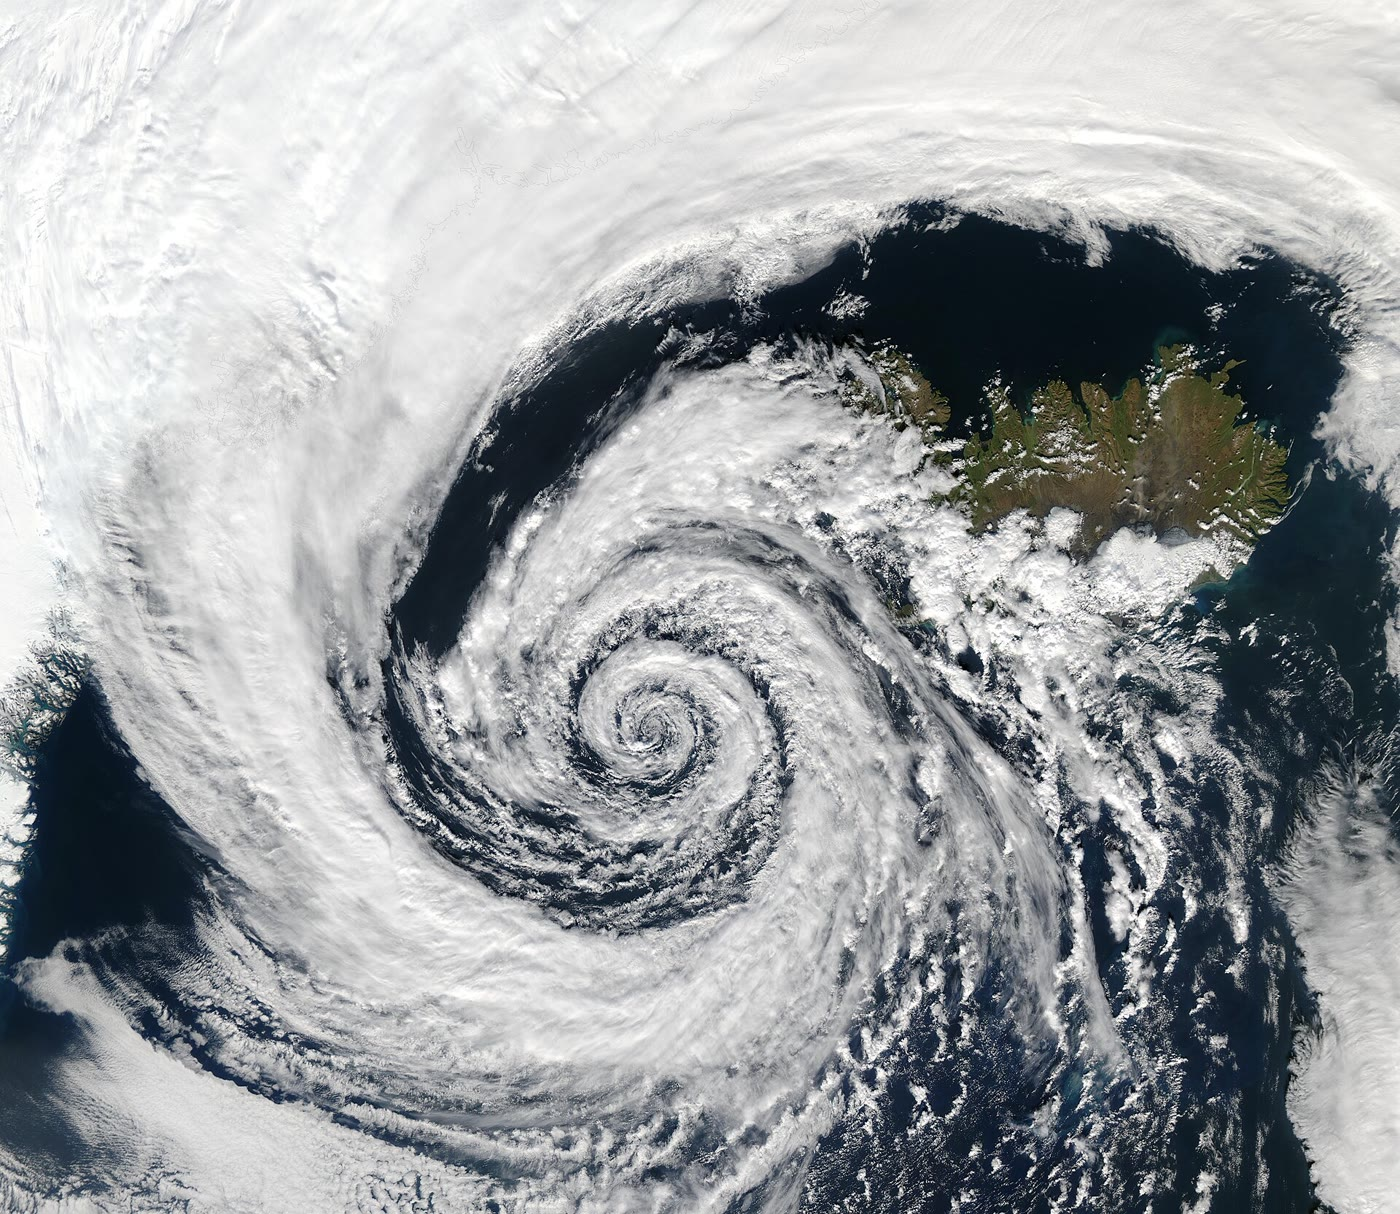
\includegraphics[width=\linewidth]{images/book5/b3-iceland-low.jpg}
\end{minipage}

\par\smallskip{\small يمينًا، معدّل نموّ إيدي بدلالة طول الموجة من أجل
قصّ متوسط كانون الثاني النطاقي عند \ang{45}~شمالًا \babelsublr{(NCEP--NCAR Reanalysis~1, 1991--2020)}،
ومتوسط التطبّق في التروبوسفير و$H = \qty{11}{km}$:
لا نموّ دون \qty{3200}{km}، وأسرع نموّ قرب \qty{4700}{km}. ويسارًا، منخفض جوي
في مرحلة نضجه قبالة الساحل الجنوبي الغربي لآيسلندا، في 4 سبتمبر 2003،
وقد التفّت سحبه في حلزون عكس اتجاه عقارب الساعة حول
المنخفض (الصورة: \mbox{\textdir TLT NASA/GSFC, MODIS Rapid Response Team}،
ملك عام).}\label{fig:b3:atmospheric-dynamics:eady}
\end{omfigure}
% ledger: data:b5-ncep-uwnd, nasa:grc-atmos, photo:b3-iceland-low

المنخفض الجوي خارج المداري الوارد في مجلد السنة الثانية هو الوجه السطحي لموجة
باروكلينية نامية: قطاعها الدافئ يحمل الهواء الدافئ نحو القطب وإلى الأعلى،
والهواء البارد خلفه ينزلق نحو خط الاستواء وإلى الأسفل، والأخدود الجوي
في الأعلى يميل غربًا مع الارتفاع، كما يقتضيه إطلاق \omterm{def:b3:atmospheric-dynamics:ape}{طاقة
الوضع المتاحة}.

\section{الدوران العام}\label{sec:b3:atmospheric-dynamics:general-circulation}

يُوصف الدوران العام بحساب المتوسط على دوائر خطوط العرض،
وما يُهمله المتوسط لا يقلّ أهمّيةً عمّا يُبقيه.

\begin{definition}[المتوسط النطاقي والاضطرابات الدوّامية]\label{def:b3:atmospheric-dynamics:eddy}
يُعرَّف \emph{المتوسط النطاقي}\index{المتوسط النطاقي} لكمية $A$ بأنّه متوسطها
على دائرة عرض عند ارتفاع أو ضغط ثابت، $[A] =
(1/2\pi)\int_0^{2\pi} A\,\mathrm d\lambda$. والانحراف $A^* = A - [A]$
هو جزؤه الدوّامي؛ و\emph{الاضطراب الدوّامي}\index{الاضطراب الدوّامي (الجوي)} في الغلاف الجوي
هو أيّ انحراف للجريان عن متوسطه النطاقي: الموجات المتنقّلة،
والموجات الثابتة، والمنخفضات والمرتفعات الجوية.
\end{definition}

يتجزّأ \omterm{def:b3:atmospheric-dynamics:eddy}{المتوسط النطاقي} لناتج الضرب إلى حدّين: $[vT] = [v][T] + [v^*T^*]$. والحدّ
الأوّل هو النقل بالدوران الطولي المتوسط، أي الخلايا الواردة في
مجلد السنة الأولى؛ والثاني هو النقل بالاضطرابات الدوّامية. وفي
خطوط العرض الوسطى تكون الريح الطولية المتوسطة ضعيفة، ويهيمن حدّ
\omterm{def:b3:atmospheric-dynamics:eddy}{الاضطراب الدوّامي}: الهواء المتحرّك نحو القطب أدفأ من الهواء المتحرّك نحو خط الاستواء
عند خط العرض نفسه، كما في الشكل أدناه، و$[v^*T^*] > 0$. وتنقل الاضطرابات الدوّامية
أيضًا زخم الريح الغربية، $[u^*v^*]$، من تحت المدارية إلى خطوط العرض
التي يقع فيها تيّار النفّاثة، وبذلك يُحافَظ على التيّار والرياح الغربية
عند السطح رغم الاحتكاك. وخليّة فيريل من مجلد السنة الأولى هي الدوران الطولي المتوسط
الذي يفرضه هذا النقل الدوّامي.

\begin{omfigure}
\begin{tikzpicture}[>=stealth, font=\small, declare function={s(\x)=0.9*sin(\x r); t(\x)=0.9*sin((\x+1.0) r);}]
\draw[thick, black, domain=0:12.566, samples=120] plot (\x, {s(\x)});
\draw[omThm, thick, densely dashed, domain=0:12.566, samples=120] plot (\x, {t(\x)-0.15});
\foreach \x in {0.3, 6.58} {\draw[->, omThm, very thick] (\x,-1.1) -- (\x,1.15)
  node[above, font=\scriptsize] {دافئ};}
\foreach \x in {3.45, 9.73} {\draw[->, omDef, very thick] (\x,1.1) -- (\x,-1.15)
  node[below, font=\scriptsize] {بارد};}
\node[font=\scriptsize, anchor=west] at (12.7,{s(12.566)}) {خط التيّار};
\node[font=\scriptsize, anchor=west, omThm] at (12.7,{t(12.566)-0.15}) {متساوي الحرارة};
\draw[->] (-1.6,-1.1) -- (-0.6,-1.1) node[below, font=\scriptsize] {شرق};
\draw[->] (-1.6,-1.1) -- (-1.6,-0.1) node[above, font=\scriptsize] {شمال};
\node[font=\scriptsize] at (6.3,-1.95) {هواء بارد نحو الشمال، ودافئ نحو الجنوب};
\end{tikzpicture}

\par\smallskip{\small موجة باروكلينية نامية في المسقط الأفقي (رسم تخطيطي،
نصف الكرة الشمالي، جريان غربي). متساوي الحرارة (المتقطّع) يتأخّر عن
خطّ التيّار بربع طول موجة أو أقلّ، فالهواء المتحرّك شمالًا (السهام
الحمراء) أدفأ من الهواء المتحرّك جنوبًا عند خط العرض نفسه (الزرقاء):
فالموجة تنقل الحرارة نحو القطب، $[v^*T^*] >
0$.}\label{fig:b3:atmospheric-dynamics:heatflux}
\end{omfigure}

في المناطق المدارية تكون الاضطرابات الدوّامية ضعيفة، ويحمل الدوران المتوسط الحرارة
نحو القطب، وهي خليّة هادلي. وجد مجلد السنة الأولى أنّ الهواء المغادر
خط الاستواء ساكنًا ويحتفظ بكمّية حركته الزاوية سيهبّ بسرعة مئات
الأمتار في الثانية عند \ang{40}، وترك مفتوحًا سببَ انتهاء الخليّة قرب
\ang{30}. يُجيب نموذج بسيط عن ذلك.

\begin{definition}[كمية الحركة الزاوية للغلاف الجوي؛ نموذج هيلد--هو]\label{def:b3:atmospheric-dynamics:held-hou}
تُعرَّف \emph{كمية الحركة الزاوية للغلاف الجوي}\index{كمية الحركة الزاوية للغلاف الجوي}
لكلّ وحدة كتلة حول محور الأرض هي $M = (\Omega a\cos\varphi +
u)\,a\cos\varphi$، لريح متجهة شرقًا $u$ عند خط العرض $\varphi$.
و\emph{نموذج هيلد--هو}\index{نموذج هيلد--هو} لخليّة هادلي هو دوران
متناظر محوريًّا ومستقرّ لغلاف جوي جافّ \omterm{def:b3:gfd-foundations:boussinesq}{بتقريب بوسينسك}، عمقه
$H$، يُسخَّن بالاسترخاء نحو درجة الحرارة الكامنة للتوازن الإشعاعي
$\theta_E/\theta_0 = 1 + \Delta/3 - \Delta\sin^2\varphi$؛ فرعه
العلوي يحفظ $M$، وفرعه السفلي ذو ريح مُهمَلة،
ويكون الجريان في توازن \omterm{thm:b3:gfd-foundations:thermal-wind}{الريح الحرارية}.
\end{definition}

\begin{theorem}[امتداد خليّة هادلي]\label{thm:b3:atmospheric-dynamics:held-hou}
في حالة الزوايا الصغيرة، تبلغ خليّة هيلد--هو خط العرض
\[
\varphi_H = \left(\frac{5\,gH\Delta}{3\,\Omega^2a^2}\right)^{1/2}
\]
في كلّ نصف كرة، وتكون ريح فرعها العلوي $u_M = \Omega
a\varphi^2$.
\end{theorem}

\begin{proof}
عند قيم $\varphi$ الصغيرة، $\cos\varphi \approx 1$، ويغادر الهواء خط الاستواء
ساكنًا بكمّية الحركة الزاوية $M = \Omega a^2$، فتكون $u_M = \Omega a(1 - \cos^2\varphi)/\cos\varphi
\approx \Omega a\varphi^2$. بوضع $f \approx 2\Omega\varphi$، $y = a\varphi$،
ومع انعدام الريح عند السطح، \omterm{thm:b3:gfd-foundations:thermal-wind}{والريح الحرارية} بصيغتها وفق \omterm{def:b3:gfd-foundations:boussinesq}{تقريب بوسينسك} على
العمق $H$، $2\Omega\varphi\,u_M/H = -(g/a\theta_0)\,\partial\theta_M/
\partial\varphi$، حيث $\theta_M$ هو المتوسط الرأسي للمقدار $\theta$ في
الخليّة. ومنه $\partial(\theta_M/\theta_0)/\partial\varphi = -2\Omega^2a^2
\varphi^3/(gH)$، و$\theta_M/\theta_0 = A - K\varphi^4$، $K = \Omega^2a^2/
(2gH)$. داخل الخليّة ينقل الدوران الحرارة دون أن يولّدها أو
يفنيها، فللخليّة متوسّط درجة الحرارة نفسه الذي في
التوازن الإشعاعي: $\int_0^{\varphi_H}\theta_M\,\mathrm d\varphi = \int_0^{\varphi_H}
\theta_E\,\mathrm d\varphi$. وعند حافّتها تكون درجة الحرارة متّصلة:
$\theta_M(\varphi_H) = \theta_E(\varphi_H)$. وبأخذ $\theta_E/\theta_0 \approx
B - \Delta\varphi^2$، $B = 1 + \Delta/3$، فيعطي الشرط الأوّل $A - B =
K\varphi_H^4/5 - \Delta\varphi_H^2/3$، والشرط الثاني $A - B = K\varphi_H^4 -
\Delta\varphi_H^2$. بالطرح، $(4/5)K\varphi_H^4 = (2/3)\Delta
\varphi_H^2$، ومنه $\varphi_H^2 = 5\Delta/(6K) = 5gH\Delta/(3\Omega^2a^2)$.
\end{proof}

تنتهي الخليّة حيث تلتقي درجة الحرارة التي يفرضها حفظ كمّية الحركة الزاوية
بالتوازن الإشعاعي؛ وما بعد ذلك يلزم أن يكون الغلاف الجوي
أبرد ممّا يجعله الإشعاع. يتضمّن النموذج معلمتين غير مرصودتين
مباشرةً. من أجل $H = \qty{15}{km}$ و$\Delta$ بين $1/6$
و$1/3$، المختارة للتوضيح، تتراوح $\varphi_H$ بين \ang{25} و\ang{35}.
أمّا الخلايا المرصودة، المستخلصة من الريح الطولية للمتوسط النطاقي، فتنتهي عند
\ang{33.3} شمالًا و\ang{32.5} جنوبًا في المتوسط السنوي، والخلايا الشتوية،
القوية منها، عند \ang{30.8} شمالًا في كانون الأوّل--شباط و\ang{29.1} جنوبًا في
حزيران--آب. والمهمّ هنا هو قانون القياس: خليّة تتّسع مع
تروبوسفير أعمق وتباين تسخين أقوى، وتضيق على
كوكب يدور أسرع. وريح الفرع العلوي للنموذج، $u_M =
\qty{88}{m/s}$ عند حافّته من أجل $\Delta = 1/6$، ضعف تيّار النفّاثة المرصود:
تُزيل الاضطرابات الدوّامية الفائض.
% ledger: geod5:grs80-defining, earth:Rmean, data:b5-ncep-vwnd (values in figdata/bachelor-3/held_hou.py)

\begin{omfigure}
\begin{tikzpicture}
\begin{groupplot}[group style={group size=2 by 1, horizontal sep=1.7cm},
  width=0.48\linewidth, height=0.44\linewidth, tick label style={font=\scriptsize},
  label style={font=\small}, legend style={font=\scriptsize, draw=none, fill=none}]
\nextgroupplot[xlabel={خط العرض \babelsublr{(\unit{\degree})}}, ylabel={\mbox{\textdir TLT $100\,(\theta/\theta_0 - 1)$}},
  xmin=0, xmax=60, ymin=-30, ymax=15, legend pos=south west, legend cell align=left,
  title={\small \mbox{\textdir TLT $\Delta = 1/3$, $H = \qty{15}{km}$}}]
% computed in figdata/bachelor-3/held_hou.py
\addplot[omDef, thick] table[x=phi, y=thE] {figdata/out/bachelor-3-held_hou-theta-3.dat};
\addplot[omThm, thick, unbounded coords=jump] table[x=phi, y=thM] {figdata/out/bachelor-3-held_hou-theta-3.dat};
\addplot[black!50, densely dashed, forget plot] coordinates {(35.26,-30) (35.26,15)};
\node[font=\scriptsize, anchor=south west] at (axis cs:35.6,7) {$\varphi_H$};
\legend{$\theta_E$, $\theta_M$}
\nextgroupplot[xlabel={خط العرض \babelsublr{(\unit{\degree})}}, ylabel={الدالة $\psi$ عند \qty{500}{hPa} \babelsublr{($10^{10}$\,\unit{kg/s})}},
  xmin=-60, xmax=60, ymin=-25, ymax=25, xtick={-60,-30,0,30,60}, legend pos=south west,
  legend cell align=left]
\addplot[black!50, thin, domain=-60:60, samples=2, forget plot] {0};
\addplot[black, thick] table[x=lat, y=ann] {figdata/out/bachelor-3-held_hou-psi.dat};
\addplot[omDef, thick] table[x=lat, y=djf] {figdata/out/bachelor-3-held_hou-psi.dat};
\addplot[omThm, thick] table[x=lat, y=jja] {figdata/out/bachelor-3-held_hou-psi.dat};
\legend{{السنوي}, {كانون الأوّل--شباط}, {حزيران--آب}}
\end{groupplot}
\end{tikzpicture}

\par\smallskip{\small يسارًا، بناء هيلد--هو: درجة الحرارة المحافظة على كمية الحركة الزاوية
للخليّة (الأحمر) تلتقي مع التوازن الإشعاعي (الأزرق) عند $\varphi_H = \ang{35}$،
مع تساوي المساحات بين المنحنيين داخل الخليّة. يمينًا، متوسط دالة الجريان الكتلي النصف-طولي
عند \qty{500}{hPa} المستخرج من الريح النصف-طولية للمتوسط النطاقي
(\babelsublr{NCEP--NCAR Reanalysis~1}، 1991--2020؛ موجبة حيث يتحرّك الهواء
فوق \qty{500}{hPa} شمالًا): تمتدّ الخليّة الشتوية القوية، في نصف الكرة
الشتوي، عبر خطّ الاستواء، وتنتهي الخلايا
بالقرب من
\ang{30}.}\label{fig:b3:atmospheric-dynamics:held-hou}
\end{omfigure}
% ledger: data:b5-ncep-vwnd

\begin{history}[من الموجات الطويلة إلى أوّل توقّع محسوب]
في عام 1939 شرع روسبي وزملاؤه، في مجلة
\emph{\babelsublr{Journal of Marine Research}}، في تفسير عدّة ظواهر تبدو مستقلّة في الطقس
من منظور واحد. ودفعته أنماط جوّية تتحرّك باتّجاه المنبع
عكس الجريان الغربي السائد، فصاغ روسبي
نظرية خطّية تميل فيها الاضطرابات الكبيرة المقياس إلى التحرّك غربًا،
والأصغر منها إلى التحرّك شرقًا نسبةً إلى الريح: الموجات والمستوي $\beta$ المذكوران في هذا الفصل.
بعد أحد عشر عامًا، حلّ تشارني وفيورتوفت وفون نويمان عدديًّا معادلةَ الدوّامية الباروتروبية
على الحاسوب الإلكتروني ENIAC: أربعة توقّعات، مدّة كلّ منها 24~ساعة، على مستوى
\qty{500}{mb}، بخطوة شبكة \qty{736}{km}، و8 درجات من خطوط الطول عند \ang{45}.
استغرق حساب كلّ توقّع نحو 24~ساعة،
وكانوا، كما كتبوا، بالكاد قادرين
على مجاراة الطقس.
\end{history}
% ledger: rossby39:paper, jmr20:commentary, charney50:eniac

\section{التمارين}

\begin{exercise}[$\star$]\label{exo:b3:atmospheric-dynamics:1}
(أ)~احسب \omterm{def:b3:atmospheric-dynamics:vorticity-kinds}{الدوّامية النسبية} لدوّامة في دوران صلب تدور
مرّةً واحدة في اليوم. (ب)~احسب \omterm{def:b3:atmospheric-dynamics:vorticity-kinds}{الدوّامية الكوكبية} عند \ang{30} و\ang{60} شمالًا
($\Omega = \qty{7.292e-5}{rad/s}$) وقارن بين النتيجتين.
\end{exercise}

\begin{exercise}[$\star$]\label{exo:b3:atmospheric-dynamics:2}
جسيم هوائي بلا دوّامية نسبية عند \ang{30} شمالًا ينتقل إلى \ang{40} شمالًا في
جريان بلا تباعد. احسب دوّاميته النسبية هناك.
هل هي حلزونية أم مضادّة للحلزون؟
\end{exercise}

\begin{exercise}[$\star$]\label{exo:b3:atmospheric-dynamics:3}
عند \ang{45} شمالًا، ومن دون ريح متوسطة، احسب سرعة الطور لموجة روسبي
ذات طول الموجة \qty{5000}{km} مع $l = 0$. في أيّ اتّجاه تتحرّك؟
\end{exercise}

\begin{exercise}[$\star$]\label{exo:b3:atmospheric-dynamics:4}
عند \ang{60} شمالًا في ريح غربية مقدارها \qty{10}{m/s}، احسب $\beta$ وطول
الموجة الثابتة وعدد الموجات الثابتة حول
دائرة خط العرض ($a = \qty{6371}{km}$).
\end{exercise}

\begin{exercise}[$\star\star$]\label{exo:b3:atmospheric-dynamics:5}
عمود هوائي بعمق \qty{10}{km}، بلا دوّامية نسبية عند \ang{45}
شمالًا، يعبر سلسلة جبلية تضغطه إلى \qty{8}{km}، ثم حوضًا يصل عمقه إلى
\qty{12}{km}. بافتراض أنّه يبقى قرب \ang{45} شمالًا، احسب دوّاميته النسبية
فوق السلسلة وفوق الحوض. أين تميل المنخفضات
إلى التشكّل؟
\end{exercise}

\begin{exercise}[$\star\star$]\label{exo:b3:atmospheric-dynamics:6}
من أجل الموجة ذات الخمسة قمم حول دائرة \ang{45} شمالًا ($l = 0$) في
ريح غربية مقدارها \qty{15}{m/s}، احسب سرعة الطور وسرعة الزمرة.
كم يستغرق انتقال طاقة الموجة مسافة \qty{5000}{km} شرقًا، وكم
يستغرق انتقال النمط ذاته؟
\end{exercise}

\begin{exercise}[$\star\star$]\label{exo:b3:atmospheric-dynamics:7}
عند \ang{45} شمالًا في ريح غربية مقدارها \qty{15}{m/s}، تكون موجة محصورة بين
خطّي عرض بحيث $l = \pi/(\qty{6000}{km})$. (أ)~احسب العدد الموجي الزونالي الثابت
وطول الموجة. (ب)~بيّن أنّه لا توجد موجة ثابتة من أجل
$l = \pi/(\qty{3000}{km})$.
\end{exercise}

\begin{exercise}[$\star\star$]\label{exo:b3:atmospheric-dynamics:8}
في \omterm{def:b3:atmospheric-dynamics:eady}{نموذج إيدي} عند \ang{45} شمالًا، $\Lambda = \qty{2e-3}{s^{-1}}$، $N =
\qty{0.012}{s^{-1}}$ و$H = \qty{10}{km}$. احسب $L_d$، ومعدّل النموّ
وزمن التضاعف الأسّي بعامل $e$ لأسرع الاضطرابات نموًّا، وطول
موجتها.
\end{exercise}

\begin{exercise}[$\star\star$]\label{exo:b3:atmospheric-dynamics:9}
على امتداد دائرة خط عرض، تكون الريح النصف-طولية للاضطراب الدوّامي $v^* = V\cos kx$
ودرجة حرارة \omterm{def:b3:atmospheric-dynamics:eddy}{الاضطراب الدوّامي} $T^* = T_0\cos(kx - \delta)$، مع $V = \qty{10}{m/s}$
و$T_0 = \qty{5}{K}$. احسب $[v^*T^*]$ من أجل $\delta = 0$، \ang{60}،
و\ang{90}، وتدفّق الحرارة المقابل $\rho c_p[v^*T^*]$ لكلّ
\unit{kg/m^3} من الهواء ($c_p = \qty{1004}{J.kg^{-1}.K^{-1}}$). أيّ
ترتيب لا ينقل حرارة؟
\end{exercise}

\begin{exercise}[$\star\star\star$]\label{exo:b3:atmospheric-dynamics:10}
انطلاقًا من \omterm{thm:b3:atmospheric-dynamics:bve}{معادلة الدوّامية الباروتروبية}، استنتج علاقة تشتّت موجات روسبي
في رياح غربية منتظمة، وبيّن أنّ كلّ موجة روسبي تتحرّك غربًا
بالنسبة إلى الهواء.
\end{exercise}

\begin{exercise}[$\star\star\star$]\label{exo:b3:atmospheric-dynamics:11}
في \omterm{def:b3:atmospheric-dynamics:held-hou}{نموذج هيلد--هو} خذ $H = \qty{12}{km}$ و$\Delta = 1/4$. احسب
$\varphi_H$، وريح الزاوية الصغيرة $u_M$ عند الحافة، وريح كمية الحركة الزاوية
الدقيقة عندها، وقارنها بالتيّار النفّاث شبه المداري البالغ
\qty{44}{m/s} للمتوسط النطاقي لشهر يناير.
\end{exercise}

\begin{exercise}[$\star\star\star$]\label{exo:b3:atmospheric-dynamics:12}
تختلف طبقتان من الهواء في درجة الحرارة الكامنة بمقدار \qty{10}{K}
عند \qty{300}{K}؛ يميل سطح فصلهما نحو القطب صعودًا بميل $s$
عبر نطاق عرضه \qty{4000}{km}، و$\rho = \qty{0.7}{kg/m^3}$. (أ)~بيّن أنّ السماح
لسطح الفصل بالتسطّح يحرّر $\rho g' s^2L^2/24$ لكلّ وحدة مساحة،
حيث $g' = g\,\Delta\theta/\theta$. (ب)~احسب ذلك من أجل $s = 10^{-3}$ و$2\times10^{-3}$
وقارنه بالطاقة الحركية لريح \qty{15}{m/s}
تعبر \qty{10}{km} من الهواء نفسه.
\end{exercise}
% ledger: geod5:grs80-defining, earth:Rmean, data:b5-ncep-uwnd

\section{مسألة: الموجة التي وقفت ساكنة}

\begin{problem}[{مسألة نهاية الأسبوع --- الدوّامية، وموجات روسبي، ونموّ
الموجة الباروكلينية عند \ang{45}~شمالًا}]
\label{pb:b3:atmospheric-dynamics:1}
يعبر جريان هوائيّ غربيّ بسرعة \qty{15}{m/s} خطوط العرض الوسطى لقارّة
متخيّلة، على امتداد \ang{45}~شمالًا. خذ $\Omega =
\qty{7.292115e-5}{rad/s}$، و$a = \qty{6371}{km}$ و$g = \qty{9.81}{m/s^2}$.
جميع قيم الجريان متخيّلة.

\medskip\noindent\textbf{الجزء الأول --- كتلة هوائية مزاحة.}
\begin{enumerate}
\item كتلة هوائية عديمة \omterm{def:b3:atmospheric-dynamics:vorticity-kinds}{الدوّامية النسبية} عند \ang{45}~شمالًا تُدفع إلى
  \ang{50}~شمالًا. احسب $f$ عند خطّي العرض، \omterm{def:b3:atmospheric-dynamics:vorticity-kinds}{والدوّامية النسبية} عند
  \ang{50}~شمالًا، إذا كان الجريان بلا تباعد.
\item متحرّكةً بسرعة \qty{15}{m/s}، على أيّ نصف قطر انحناء تنعطف؟
  (خذ $\zeta = -V/R$، على أنّ كلّها ناتج عن الانحناء)؟ في أيّ اتّجاه تنعطف؟
\item إذا انكمش عمودها أيضًا من \qty{10.0}{km} إلى \qty{9.5}{km} في أثناء
  الطريق، فما دوّاميتها النسبية عند \ang{50}~شمالًا؟
\item إذا دُفعت بدلًا من ذلك إلى \ang{40}~شمالًا، دون تباعد، فما \omterm{def:b3:atmospheric-dynamics:vorticity-kinds}{الدوّامية النسبية}
  التي تكتسبها؟ اشرح لماذا تتذبذب
  كتلةٌ هوائية أُزيحت عن خطّ عرضها حولَه.
\end{enumerate}

\medskip\noindent\textbf{الجزء الثاني --- الموجات المتنقّلة.}
\begin{enumerate}[resume]
\item احسب $\beta$ عند \ang{45}~شمالًا وطول دائرة خط العرض.
\item من أجل $n = 3$ إلى 8 موجات حول الدائرة ($l = 0$)، احسب طول الموجة،
  وسرعة الطور، وسرعة المجموعة في الرياح الغربية البالغة
  \qty{15}{m/s}.
\item أيّ الموجات تتحرّك غربًا، وأيّ منها شرقًا؟ كم يومًا تستغرق الموجة
  $n = 5$ لتقطع \qty{1000}{km}؟
\item تشتدّ الظهرة فوق غرب القارّة. أين، وبعد كم من الزمن،
  سيبلغ أثر الموجة $n = 6$ مسافة \qty{5000}{km}
  في اتّجاه الجريان؟
\end{enumerate}

\medskip\noindent\textbf{الجزء الثالث --- الموجة التي وقفت ساكنة.}
\begin{enumerate}[resume]
\item احسب طول الموجة الثابتة وعدد الموجة الثابتة عند
  \ang{45}~شمالًا.
\item احسب عدد الموجة الثابتة من أجل رياح غربية بسرعتَي 10 و\qty{20}{m/s}.
  ماذا يحدث للموجات الثابتة عندما تشتدّ الرياح الغربية
  في الشتاء؟
\item احسب عدد الموجة الثابتة عند \ang{35}~شمالًا و\ang{55}~شمالًا في
  الرياح الغربية البالغة \qty{15}{m/s}.
\item ترتفع الجبال الغربية للقارّة \qty{2}{km} داخل التروبوسفير
  التي يبلغ عمقها \qty{10}{km}. احسب \omterm{def:b3:atmospheric-dynamics:vorticity-kinds}{الدوّامية النسبية} لعمود يعبر
  هذه الجبال دون أن يتغيّر خطّ عرضه.
  لماذا تفرض الجبال موجات ثابتة؟
\item لماذا لا يظلّ نمط الموجة الذي تفرضه الجبال ساكنًا
  إلّا عندما يكون طول موجته قريبًا من $\lambda_s$؟
\end{enumerate}

\medskip\noindent\textbf{الجزء الرابع --- عاصفة تتعاظم.}
\begin{enumerate}[resume]
\item تزداد الرياح الغربية من سطح الأرض حتى \qty{10}{km} بمقدار
  \qty{25}{m/s}. احسب القصّ $\Lambda$، وتدرّج درجة الحرارة نحو القطب الذي
  يقتضيه \omterm{thm:b3:gfd-foundations:thermal-wind}{بالريح الحرارية} عند متوسط درجة حرارة
  \qty{250}{K}.
\item مع $N = \qty{0.011}{s^{-1}}$، احسب عدد ريتشاردسون
  $N^2/\Lambda^2$. هل الجريان غير مستقرّ أمام اضطراب القصّ صغير المقياس؟
\item احسب نصف قطر روسبي $L_d$ من أجل $H = \qty{10}{km}$.
\item احسب طول موجة الاضطراب الأسرع نموًّا في \omterm{def:b3:atmospheric-dynamics:eady}{نموذج إيدي}، وعدد هذه الموجات
  حول دائرة خط العرض.
\item احسب أقصر طول موجة ينمو.
\item احسب معدّل النموّ $\sigma_{\max}$.
\item بأيّ عامل ينمو الاضطراب خلال ثلاثة أيّام؟
\item قارن طول موجة العاصفة النامية بطول الموجة الثابتة في الجزء~الثالث:
  أيّهما أطول، وماذا يعني ذلك لحركة العواصف بالنسبة إلى الموجات
  الثابتة؟
\item في أيّ اتّجاه يميل قاعُ الموجة النامية مع الارتفاع،
  ولماذا يجب أن يكون كذلك؟
\item أعطِ زمن الزيادة بعامل $e$ للاضطراب الأسرع نموًّا في \omterm{def:b3:atmospheric-dynamics:eady}{نموذج إيدي}.
\end{enumerate}
\end{problem}
% ledger: geod5:grs80-defining, earth:Rmean
